\documentclass[a4paper,
fontsize=11pt,
%headings=small,
oneside,
numbers=noperiodatend,
parskip=half-,
bibliography=totoc,
final
]{scrartcl}

\usepackage[babel]{csquotes}
\usepackage{synttree}
\usepackage{graphicx}
\setkeys{Gin}{width=.4\textwidth} %default pics size

\graphicspath{{./plots/}}
\usepackage[ngerman]{babel}
\usepackage[T1]{fontenc}
%\usepackage{amsmath}
\usepackage[utf8x]{inputenc}
\usepackage [hyphens]{url}
\usepackage{booktabs} 
\usepackage[left=2.4cm,right=2.4cm,top=2.3cm,bottom=2cm,includeheadfoot]{geometry}
\usepackage[labelformat=empty]{caption} % option 'labelformat=empty]' to surpress adding "Abbildung 1:" or "Figure 1" before each caption / use parameter '\captionsetup{labelformat=empty}' instead to change this for just one caption
\usepackage{array}
\usepackage{eurosym}
\usepackage{multirow}
\usepackage[ngerman]{varioref}
\setcapindent{1em}
\renewcommand{\labelitemi}{--}
\usepackage{paralist}
\usepackage{pdfpages}
\usepackage{lscape}
\usepackage{float}
\usepackage{acronym}
\usepackage{eurosym}
\usepackage{longtable,lscape}
\usepackage{mathpazo}
\usepackage[normalem]{ulem} %emphasize weiterhin kursiv
\usepackage[flushmargin,ragged]{footmisc} % left align footnote
\usepackage{ccicons} 
\setcapindent{0pt} % no indentation in captions

%%%% fancy LIBREAS URL color 
\usepackage{xcolor}
\definecolor{libreas}{RGB}{112,0,0}

\usepackage{listings}

\urlstyle{same}  % don't use monospace font for urls

\usepackage[fleqn]{amsmath}

%adjust fontsize for part

\usepackage{sectsty}
\partfont{\large}

%Das BibTeX-Zeichen mit \BibTeX setzen:
\def\symbol#1{\char #1\relax}
\def\bsl{{\tt\symbol{'134}}}
\def\BibTeX{{\rm B\kern-.05em{\sc i\kern-.025em b}\kern-.08em
    T\kern-.1667em\lower.7ex\hbox{E}\kern-.125emX}}

\usepackage{fancyhdr}
\fancyhf{}
\pagestyle{fancyplain}
\fancyhead[R]{\thepage}

% make sure bookmarks are created eventough sections are not numbered!
% uncommend if sections are numbered (bookmarks created by default)
\makeatletter
\renewcommand\@seccntformat[1]{}
\makeatother

% typo setup
\clubpenalty = 10000
\widowpenalty = 10000
\displaywidowpenalty = 10000

\usepackage{hyperxmp}
\usepackage[colorlinks, linkcolor=black,citecolor=black, urlcolor=libreas,
breaklinks= true,bookmarks=true,bookmarksopen=true]{hyperref}
\usepackage{breakurl}

%meta
%meta

\fancyhead[L]{Strecker, D.\\ %author
LIBREAS. Library Ideas, 42 (2022). % journal, issue, volume.
%\href{https://doi.org/10.18452/...}{\color{black}https://doi.org/10.18452/...}
{}} % doi 
\fancyhead[R]{\thepage} %page number
\fancyfoot[L] {\ccLogo \ccAttribution\ \href{https://creativecommons.org/licenses/by/4.0/}{\color{black}Creative Commons BY 4.0}}  %licence
\fancyfoot[R] {ISSN: 1860-7950}

\title{\LARGE{Dataset Retrieval: Informationsverhalten von Datensuchenden und das Ökosystem von Data-Retrieval-Systemen}}% title
\author{Dorothea Strecker} % author

\setcounter{page}{1}

\hypersetup{%
      pdftitle={Dataset Retrieval: Informationsverhalten von Datensuchenden und das Ökosystem von Data-Retrieval-Systemen},
      pdfauthor={Dorothea Strecker},
      pdfsubject={LIBREAS. Library Ideas, 42 (2022).},
      pdfkeywords={Forschungsdaten, Suche, Datenveröffentlichung, research data, published data, dataset, retrieval},
      pdflicenseurl={https://creativecommons.org/licenses/by/4.0/},
      pdfcopyright={CC BY 4.0 International},
      pdfcontacturl={http://libreas.eu},
      pdfurl={https://doi.org/10.18452/...},
      pdfdoi={10.18452/...},
      pdflang={de},
      pdfmetalang={de}
     }



\date{}
\begin{document}

\maketitle
\thispagestyle{fancyplain} 

%abstracts
\begin{abstract}
\noindent
\textbf{Kurzfassung}: Verschiedene Stakeholder fordern eine bessere
Verfügbarkeit von Forschungsdaten. Der Erfolg dieser Initiativen hängt
wesentlich von einer guten Auffindbarkeit der publizierten Datensätze
ab, weshalb Dataset Retrieval an Bedeutung gewinnt. Dataset Retrieval
ist eine Sonderform von Information Retrieval, die sich mit dem
Auffinden von Datensätzen befasst. Dieser Beitrag fasst aktuelle
Forschungsergebnisse über das Informationsverhalten von Datensuchenden
zusammen. Anschließend werden beispielhaft zwei Suchdienste
verschiedener Ausrichtung vorgestellt und verglichen. Um darzulegen, wie
diese Dienste ineinandergreifen, werden inhaltliche Überschneidungen von
Datenbeständen genutzt, um den Metadatenaustausch zu analysieren.

\noindent
\textbf{Abstract}: Various stakeholders are calling for better
availability of research data. The success of these initiatives depends
largely on good discoverability of published datasets, which is why
Dataset Retrieval is gaining in importance. Dataset Retrieval is a
special form of Information Retrieval that is concerned with finding
datasets. This paper summarizes recent research on the information
behavior of data users. Subsequently, two search services with different
objectives are presented and compared. In order to show how these
services interconnect, overlaps in content are used to analyze metadata
exchange between them.
\end{abstract}

%body
\hypertarget{einleitung}{%
\section{Einleitung}\label{einleitung}}

Um die Nachvollziehbarkeit und Nachnutzbarkeit von Forschungsergebnissen
zu fördern, fordern verschiedene Stakeholder eine bessere Verfügbarkeit
von Forschungsdaten. Der Erfolg dieser Initiativen hängt allerdings
wesentlich von einer guten Auffindbarkeit der publizierten Datensätze
ab, denn der Kreis von der Publikation bis zur Nachnutzung bestehender
Forschungsdaten lässt sich nur schließen, wenn für die jeweilige
Fragestellung passende Daten gefunden werden können.

Verschiedene Aspekte von Information Retrieval werden schon lange
beforscht, inzwischen hat sich ein eigenständiges Forschungsfeld
etabliert (Luk 2022). Im Zuge der wachsenden Anzahl publizierter
Forschungsdaten kommen auch Retrieval-Systeme auf, die sich auf das
Auffinden von Forschungsdaten spezialisiert haben. Diese Entwicklung
bringt neue Fragestellungen und Herausforderungen mit sich.

Beispielsweise müssen Informationsbedürfnisse und -verhalten von
Datensuchenden analysiert werden, um bedarfsgerechte Angebote entwickeln
zu können. Außerdem muss sich ein stabiles Ökosystem von Suchdiensten
entwickeln, die variierende Bestände durchsuchbar machen, wie es
beispielsweise im Bibliotheksbereich schon lange existiert.

\hypertarget{fragestellungen}{%
\subsection{Fragestellungen}\label{fragestellungen}}

In diesem Beitrag soll darum dargestellt werden, was aktuell über das
Informationsverhalten von Datensuchenden bekannt ist. Anschließend
werden beispielhaft zwei Suchdienste -- PANGAEA und Google Dataset
Search -- mit besonderem Fokus auf Unterschiede in ihrer Datengrundlage
und Funktionsweise vorgestellt. Um zu zeigen, wie diese Dienste
ineinandergreifen, werden inhaltliche Überschneidungen von
Datenbeständen genutzt, um den Metadatenaustausch zu analysieren.

\hypertarget{literaturuxfcbersicht}{%
\section{Literaturübersicht}\label{literaturuxfcbersicht}}

\hypertarget{information-retrieval-und-dataset-retrieval}{%
\subsection{Information Retrieval und Dataset
Retrieval}\label{information-retrieval-und-dataset-retrieval}}

Allgemein bezeichnet Information Retrieval (IR) den Prozess, bei dem
gezielt nach Informationsobjekten in einer Sammlung gesucht wird, die
ein bestimmtes Informationsbedürfnis abdecken (Meadow et al.~2007).
Systeme, die IR ermöglichen, repräsentieren und organisieren
Informationen auf unterschiedliche Weise, um sie durchsuchbar zu machen,
und bieten verschiedene Einstiege für die Suche an. Die Ursprünge von IR
sind eng mit der Entwicklung des Bibliothekswesens verknüpft (Sanderson
und Croft 2012). Im Laufe der Zeit haben sich IR-Systeme wesentlich
weiterentwickelt, und IR hat sich als eigenständige Forschungsdisziplin
etabliert (Luk 2022).

Dataset Retrieval (DR) kann als Sonderform von IR betrachtet werden, die
sich auf das Auffinden von Informationsobjekten eines besonderen Typs
(Datensätze) spezialisiert (Chen et al.~2019; Kunze und Auer 2013). DR
ist ein vergleichsweise neues Forschungsfeld, das sich in der
Anfangszeit vorwiegend mit technischen Herausforderungen beschäftigt
hat; soziale Aspekte wie Informationsbedürfnisse und -verhalten wurden
erst in den letzten Jahren systematisch beforscht (Gregory, Cousijn, et
al.~2020). Diese Aspekte sind jedoch wichtig, um das
Informationsverhalten von Datensuchenden zu verstehen und daraus
Anforderungen an DR-Systeme abzuleiten.

\hypertarget{funktionsweise-von-dr-systemen}{%
\subsection{Funktionsweise von
DR-Systemen}\label{funktionsweise-von-dr-systemen}}

Grundsätzlich funktionieren DR-Systeme wie andere IR-Systeme: Eine
Anfrage durch Nutzende erfolgt in den Phasen \emph{querying} (Stellen
der Anfrage durch den*die Nutzer*in), \emph{query handling} (Bearbeitung
der Anfrage durch den Suchdienst), \emph{data handling} (Identifizieren
von Treffern durch den Suchdienst) und \emph{results presentation}
(Anzeigen der Treffer durch den Suchdienst) (Chapman et al.~2020). Das
DR-System erstellt im Voraus einen Index der durchsuchbaren Dokumente
und beinhaltet Komponenten, die Anfragen mit dem Index abgleichen und
Trefferlisten erstellen (Chen et al.~2019). Der Index kann auf
verschiedene Weise erzeugt werden, beispielsweise durch das gezielte
Harvesten von Metadaten über die Schnittstellen ausgewählter Dienste
oder durch Crawls, die regelmäßig eine große Zahl von Repositorien
ansteuern (Chapman et al.~2020). DR basiert aktuell überwiegend auf
strukturierten Metadaten, die Repositorien bereitstellen (Chapman et al.
2020; Devaraju und Berkovsky 2018). Ansätze zur Anreicherung des Indexes
wie die Volltextindexierung von Publikationen, die auf den
durchsuchbaren Datensätzen aufbauen, sind bisher noch wenig verbreitet
(Khalsa, Cotroneo, und Wu 2018).

Aktuell sind die Suchfunktionalitäten von DR-Systemen vorwiegend auf
Keywordsuche und facettierte Navigation beschränkt (Devaraju und
Berkovsky 2018). Um den Ansprüchen von Nutzenden gerecht zu werden,
sollten Repositorien möglichst mehrere Sucheinstiege anbieten,
beispielsweise neben einem einfachen Suchschlitz auch eine erweiterte
Suche, die Suche über eine Karte oder Browsing nach Facetten (Wu et al.
2019) -- was viele Repositorien bereits umgesetzt haben (Khalsa,
Cotroneo, und Wu 2018).

\hypertarget{evaluation-von-dr-systemen}{%
\subsection{Evaluation von
DR-Systemen}\label{evaluation-von-dr-systemen}}

Ein ungelöstes Problem ist die Evaluation von DR-Systemen. In einer
Umfrage von 2018 unter 98 Repositorienbetreiber*innen gab nur etwa ein
Drittel der Befragten an, das DR-System in der Vergangenheit evaluiert
zu haben, und nur etwa die Hälfte war sich sicher, dass die meisten
Anfragen durch das System für Nutzer*innen zufriedenstellend beantwortet
werden (Khalsa, Cotroneo, und Wu 2018). Ein Grund dafür könnte sein,
dass verbreitete Metriken und Benchmarks für die Evaluation von
IR-Systemen häufig auf Textdokumente ausgelegt sind und nicht immer
direkt auf Datensätze übertragbar sind (Chapman et al.~2020).

Trotz dieser Herausforderungen gibt es einige Publikationen, die Aspekte
von DR-Systemen evaluieren. So zeigte sich beispielsweise, dass die
Relevanzbewertung von Treffern noch besser an spezifische Besonderheiten
von Datensätzen angepasst werden könnte (Dede Şener, Ogul, und Basak
2022). Auch verschiedene Ansätze für Recommender-Services, die ähnliche
Datensätze aufzeigen, wurden erprobt (Wang, Huang, und Harmelen 2020).

Es gibt erste Hinweise darauf, dass integrierte Retrieval-Systeme, die
sowohl Daten- und Textpublikationen auffindbar machen, unterschiedlich
gut mit diesen Dokumenttypen umgehen. In einem solchen integrierten
System waren einige populäre Datensätze sehr gut, viele andere dagegen
weniger gut auffindbar (Roy, Carevic, und Mayr 2022). Die Auffindbarkeit
bei Textpublikationen war im Vergleich gleichmäßiger verteilt, außerdem
führte die Suche nach Textpublikationen wesentlich häufiger zu direkten
Interaktionen mit Inhalten.

\hypertarget{informationsverhalten-im-kontext-von-forschungsdaten}{%
\subsection{Informationsverhalten im Kontext von
Forschungsdaten}\label{informationsverhalten-im-kontext-von-forschungsdaten}}

Borst und Limani (2020) stellen \emph{data search} als dreiteiliges
Konzept dar, das die Aspekte \emph{discovery} (Suche nach Datensätzen in
einem Retrievalsystem), \emph{exploration} (Inhalt und Struktur eines
Datensatzes mithilfe der Metadaten erkunden) und \emph{analysis} (Teile
eines Datensatzes gemäß einer Fragestellung und datensatzspezifischer
Eigenschaften auswählen) umfasst. In diesem Beitrag wird vorwiegend der
Aspekt \emph{discovery} behandelt.\\

Forschende suchen Daten für diverse Nachnutzungsszenarien (Gregory et
al.~2019). Diese lassen sich grob in \emph{background}-Nutzung (wie etwa
die Kalibrierung von Messinstrumenten oder den Einsatz von Daten in der
Lehre) und \emph{foreground}-Nutzung (wie etwa das Beantworten eigener,
neuer Fragestellungen anhand nachgenutzter Daten) unterteilen (Gregory,
Cousijn, et al.~2020).

Aktuell basieren DR-Ansätze überwiegend auf Erfahrungen mit der Suche
nach Textdokumenten (Borst und Limani 2020). Die Suche nach Daten
unterscheidet sich jedoch in einigen zentralen Aspekten von der Suche
nach Textpublikationen. So sind Daten im Vergleich komplexere Objekte,
da sie auch Begleitmaterial wie Codebücher beinhalten können (Carevic,
Roy, und Mayr 2020). Zudem sind die Anforderungen an DR deutlich
vielfältiger: DR-Systeme werden je nach Informationsbedürfnis auch mit
Aspekten wie Provenienz, Qualität, Granularität und Interoperabilität
von Daten konfrontiert (Chapman et al.~2020). Darum werden Metadaten bei
DR wichtiger eingeschätzt, da Forschende über Metadaten den Kontext der
Daten verstehen und die Nutzbarkeit bewerten können (Kern und Mathiak
2015).

\hypertarget{suchstrategien}{%
\subsubsection{Suchstrategien}\label{suchstrategien}}

In einer Umfrage von 2020 unter 1.677 Forschenden berichtete die
Mehrzahl der Befragten, dass sie die Suche nach Daten herausfordernd
oder sogar schwierig finden; ein Drittel gab als Grund dafür
unzureichende Suchdienste an (Gregory, Groth, et al.~2020). Forschende
nutzen für das Auffinden von Datensätzen verschiedene Quellen und
Strategien. Häufig genutzt werden beispielsweise persönliche Kontakte,
Verweise in Textpublikationen oder Websuchmaschinen (Friedrich 2020;
Gregory, Groth, et al.~2020; Krämer et al.~2021). Die Nutzung
spezialisierter Dienste wie Forschungsdatenrepositorien oder
Suchmaschinen für Forschungsdaten ist demgegenüber weniger verbreitet
(Gregory, Groth, et al.~2020). Insbesondere zu Beginn eines
Suchprozesses nutzen Forschende häufig Websuchmaschinen, sowohl um
Daten- oder Textpublikationen als auch um spezialisierte Angebote für
die Datensuche zu finden (Krämer et al.~2021). Allgemeine
Berufserfahrung scheint einen positiven Einfluss auf die Diversität der
Quellen zu haben, die Forschende für DR nutzen (Friedrich 2020). Eine
erste Metaanalyse zeigt, dass sich die Informationsbedürfnisse und
Herausforderungen von Forschenden und Forschungsdatenexpert*innen wie
Data Librarians, ähneln (Sun et al.~2022). Allerdings nutzen sie
unterschiedliche Strategien, um geeignete Daten zu finden -- so nutzen
Data Librarians weniger häufig Websuchmaschinen.

Wenn Forschende Websuchmaschinen für DR nutzen, ergänzen sie die
Suchanfrage häufig um Begriffe wie \enquote*{data} oder
\enquote*{dataset}, um ihr Bedürfnis zu präzisieren (Koesten et
al.~2017; Krämer et al.~2021). Websuchmaschinen spielen auch eine
wichtige Rolle beim Auffinden spezialisierter Datensuchdienste. Die
Logfiles von Open-Data-Portalen zeigen beispielsweise, dass die meisten
Nutzer*innen über Websuchmaschinen auf die Seiten der Portale gelangten
(Kacprzak et al. 2019; Koesten et al.~2017). Obwohl viele Nutzer*innen
die Open-Data-Portale und ihre Inhalte bereits kannten, was die gehäufte
Nennung dieser Portale in den Anfragen an Websuchmaschinen nahelegt,
zogen sie offenbar die Suchfunktion der Websuchmaschinen den
Open-Data-Portalen vor. Nutzer*innen, die von externen Diensten wie
Websuchmaschinen auf Inhalte von Open-Data-Portalen verwiesen wurden,
brachen ihre Suche allerdings auch schneller erfolglos ab als
Nutzer*innen, die den gesamten Suchprozess im Portal durchführten
(Ibáñez und Simperl 2022).

Im Vergleich zu Suchanfragen an Websuchmaschinen sind Suchanfragen an
spezialisierte Datensuchdienste in der Tendenz kürzer. Suchanfragen an
Open-Data-Portale umfassten im Durchschnitt beispielsweise zwischen 1,63
und 2,52 Wörter (Kacprzak et al.~2017). Forschende scheinen kurze
Suchanfragen bewusst einzusetzen, um lange Trefferlisten zu erstellen,
die sie dann manuell auf Nutzbarkeit überprüfen (Kacprzak et al.~2019;
Koesten et al.~2017). Beim DR über spezialisierte Datensuchdienste
enthalten Suchanfragen außerdem häufiger Ziffern, räumliche oder
zeitliche Einschränkungen in verschiedenen Granularitätsstufen oder die
Nennung spezieller Datentypen oder -formate (Carevic, Roy, und Mayr
2020; Kacprzak et al.~2019). Suchanfragen an Datensuchdienste scheinen
insgesamt ein breiteres Spektrum von Themen abzudecken (Kacprzak et al.
2019). Bei der Suche nach Daten sind sich Suchanfragen, die innerhalb
einer Session gestellt werden, thematisch ähnlicher als bei der Suche
nach Textpublikationen (Carevic, Roy, und Mayr 2020). Interaktionspfade
bei der Suche nach Daten- und Textpublikationen ähneln sich generell,
allerdings werden Anfragen bei der Suche nach Textpublikationen häufiger
umformuliert und neu gestellt (Carevic, Roy, und Mayr 2020).

Unklar ist noch, in welchem Umfang \emph{known-item search} auftritt --
die Suche nach einem bestimmten, bereits bekannten Datensatz. Dass beim
DR explorative Ansätze verfolgt werden, zeigt sich beispielsweise daran,
dass Suchende durch kurze Suchanfragen bewusst lange Trefferlisten
erzeugen (Kacprzak et al.~2017, 2019). Jedoch gibt es keine Einigkeit
über die Verbreitung von \emph{known-item search}: Analysen zeigen, dass
Anfragen an spezialisierte Datensuchdienste selten angepasst und
verändert neu gestellt werden (Koesten et al.~2017; Carevic, Roy, und
Mayr 2020). In diesem Bereich ist mehr Forschung erforderlich, um
\emph{known-item search} in DR-Systemen besser unterstützen zu können.

Die hier beschriebenen Studien des Informationsverhaltens in Bezug auf
DR legen nahe, dass es bisher kaum einheitliche und bewährte Strategien
für die Suche nach Datensätzen gibt (Krämer et al.~2021).

\hypertarget{arten-von-dr-systemen}{%
\subsection{Arten von DR-Systemen}\label{arten-von-dr-systemen}}

Grundlegend gibt es verschiedene Arten von DR-Systemen. Sie bilden ein
komplexes Ökosystem, in dem jeder Dienst abhängig von der Mission und
Nutzer*innengruppe verschiedene Bedürfnisse abdeckt. Beispielsweise
können DR-Systeme in zentrale und dezentrale Angebote unterteilt werden
(Chapman et al.~2020). Sie divergieren darin, ob ein zentraler Bestand
durchsuchbar gemacht wird oder ob Inhalte mehrerer Quellen
zusammengeführt werden (Borst und Limani 2020). Suchdienste
unterscheiden sich außerdem in ihrem disziplinären Fokus:
Disziplinübergreifende Angebote machen Bestände mehrerer Disziplinen
durchsuchbar, während sich disziplinspezifische DR-Systeme auf Daten
einer Disziplin konzentrieren.\\
Im Folgenden werden beispielhaft zwei DR-Systeme vorgestellt und
verglichen, die verschiedenen Ansätzen folgen. Google Dataset Search,
ein sehr umfassender dezentraler und disziplinübergreigender Dienst,
wird PANGAEA, einem zentralen und disziplinspezifischen Dienst
gegenübergestellt.

\hypertarget{dezentral-und-disziplinuxfcbergreifend-google-dataset-search}{%
\subsubsection{Dezentral und disziplinübergreifend: Google Dataset
Search}\label{dezentral-und-disziplinuxfcbergreifend-google-dataset-search}}

2018 wurde Google Dataset Search in der Beta-Version veröffentlicht. Der
Dienst nahm 2020 offiziell den Betrieb auf (Noy und Benjelloun 2020).

\textbf{Datenquellen:} Der Index von Google Dataset Search basiert zwar
auf Crawls, im Gegensatz zur Google Websuchmaschine aber zugleich auf
strukturierten Metadaten. Datenlieferanten zeichnen Metadaten nach
bestimmten Standards (schema.org und DCAT) aus und stellen diese
strukturierten Metadaten über die landing pages individueller Datensätze
zur Verfügung. Ein Crawler sammelt diese Metadaten, die anschließend
verarbeitet und indexiert werden. Anfragen von Nutzenden werden mit dem
Index abgeglichen und Ergebnisse nach Relevanz sortiert angezeigt. Die
Relevanzbewertung basiert auf demselben Ansatz wie die Google
Websuchmaschine, bezieht jedoch auch Aspekte von Metadatenqualität ein
(Brickley, Burgess, und Noy 2019).\\
Die Größenverteilung der Datenquellen in Google Dataset Search ist stark
verzerrt: Die 20 größten Datenlieferanten machen 78\,\% des gesamten
Bestands aus (Benjelloun, Chen, und Noy 2020). Welche Inhalte der Google
Dataset Search Index im Detail umfasst, ist unbekannt. Google Dataset
Search indexiert auch Aggregatoren von Metadaten, beispielsweise
DataCite. Das führt dazu, dass die Registrierung von DOIs neben anderen
Vorteilen auch als Strategie empfohlen wird, um Datensätze über Google
Dataset Search auffindbar zu machen (Masson et al.~2021).

\textbf{Metadaten:} Da der Dienst disziplinübergreifend konzipiert ist,
ist das verwendete Metadatenschema sehr generisch. Außerdem gibt es nur
zwei Pflichtfelder: Titel und Beschreibung. Daraus ergeben sich Probleme
in Bezug auf die Metadatenqualität, insbesondere die Vollständigkeit. So
sind beispielsweise Lizenzinformationen nur für 34\,\% der Datensätze
verfügbar (Benjelloun, Chen, und Noy 2020).

\textbf{Sucheinstiege:} Der Sucheinstieg bei Google Dataset Search ist
auf eine einfache Keywordsuche beschränkt, auch die Präsentation der
Ergebnisse ist einfach gehalten. Eine niedrigschwellige Anwendung muss
jedoch kein Nachteil sein, sondern könnte die Nachnutzung von Daten
popularisieren und Anreize für das Publizieren von Datensätzen schaffen
(Canino 2019).

\textbf{Ergebnispräsentation:} Ergebnisse werden in Google Dataset
Search mit den vorhandenen Metadaten dargestellt (siehe Abbildung 1).
Sofern vorhanden, wird die räumliche Abdeckung des Datensatzes auf einer
Karte gezeigt.

\begin{figure}
\centering
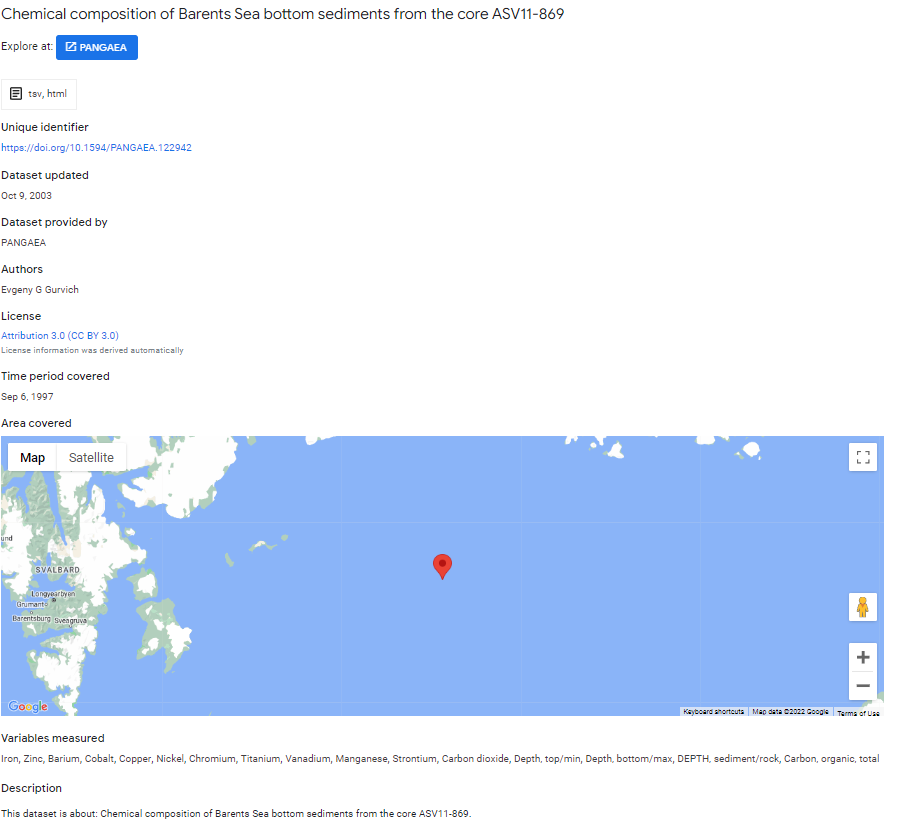
\includegraphics[width=.6\textwidth]{img/abb1_GDS_results.png}
\caption{Abbildung 1: Ergebnispräsentation für den Datensatz
\url{https://doi.org/10.1594/PANGAEA.122942} in Google Dataset Search}
\end{figure}

\hypertarget{zentral-und-disziplinspezifisch-pangaea}{%
\subsubsection{Zentral und disziplinspezifisch:
PANGAEA}\label{zentral-und-disziplinspezifisch-pangaea}}

PANGAEA nahm 1994 den Betrieb auf. Das disziplinspezifische
Forschungsdatenrepositorium hat sich auf das Publizieren
georeferenzierter Datensätze aus Bereichen der Erdsystemwissenschaft
spezialisiert (Diepenbroek et al.~2002).

\textbf{Datenquellen:} Der Suchdienst umfasst die in PANGAEA
publizierten Datensätze.\footnote{PANGAEA Terms of Use:
  \url{https://www.pangaea.de/about/terms.php}}

\textbf{Metadaten:} Metadaten in PANGAEA sind an die spezifischen
Besonderheiten der publizierten Datensätze angepasst. So bietet das
Format, das zur Beschreibung von Datensätzen genutzt wird, die
Möglichkeit, detaillierte Informationen zu dem dokumentierten Ereignis,
Expeditionen und den Erhebungsmethoden anzugeben (Diepenbroek et al.
2017). Umfassende Kurations- und Qualitätssicherungsprozesse stellen die
Nützlichkeit der Metadaten sicher.\\
PANGAEA macht Metadaten offen (unter einer CC0-Lizenz) über
Schnittstellen\footnote{Es werden verschiedene Schnittstellen angeboten,
  siehe die API-Dokumentation: \textless https://ws.pangaea.de/}
zugänglich. Der Dienst legt Wert auf die Interoperabilität der Metadaten
und liefert sie in entsprechenden Formaten an verschiedene Aggregatoren
aus, beispielsweise GBIF oder OpenAIRE. Metadaten werden außerdem nach
schema.org ausgezeichnet über die landing pages bereitgestellt. Diese
Aktivitäten führen dazu, dass die publizierten Datensätze auch in
anderen dezentralen DR-Systemen gut auffindbar sind.

\textbf{Sucheinstiege:} PANGAEA bietet neben einer einfachen
Keywordsuche auch Browsing nach Disziplinen und über eine Karte an. Das
PANGAEA Data Warehouse ermöglicht Datennutzenden außerdem das effiziente
Zusammenstellen von Datensätzen nach selbst definierten Parametern wie
beispielsweise alle Messungen einer bestimmten Größe für eine
Region.\footnote{PANGAEA Data Warehouse:
  \url{https://www.pangaea.de/tools/}}

\textbf{Ergebnispräsentation:} PANGAEA stellt den Kontext von
Datensätzen beispielsweise durch Details zur Datenerhebung oder Projekte
und andere Publikationen, die mit dem Datensatz in Zusammenhang stehen
(siehe Abbildung 2), sehr ausführlich dar. Die räumliche Abdeckung des
Datensatzes wird auf einer Karte abgebildet. Außerdem werden
Zitationsempfehlung, Ansichts- und Downloadzahlen sowie eine Übersicht
der im Datensatz enthaltenen Variablen angezeigt.

\begin{figure}
\centering
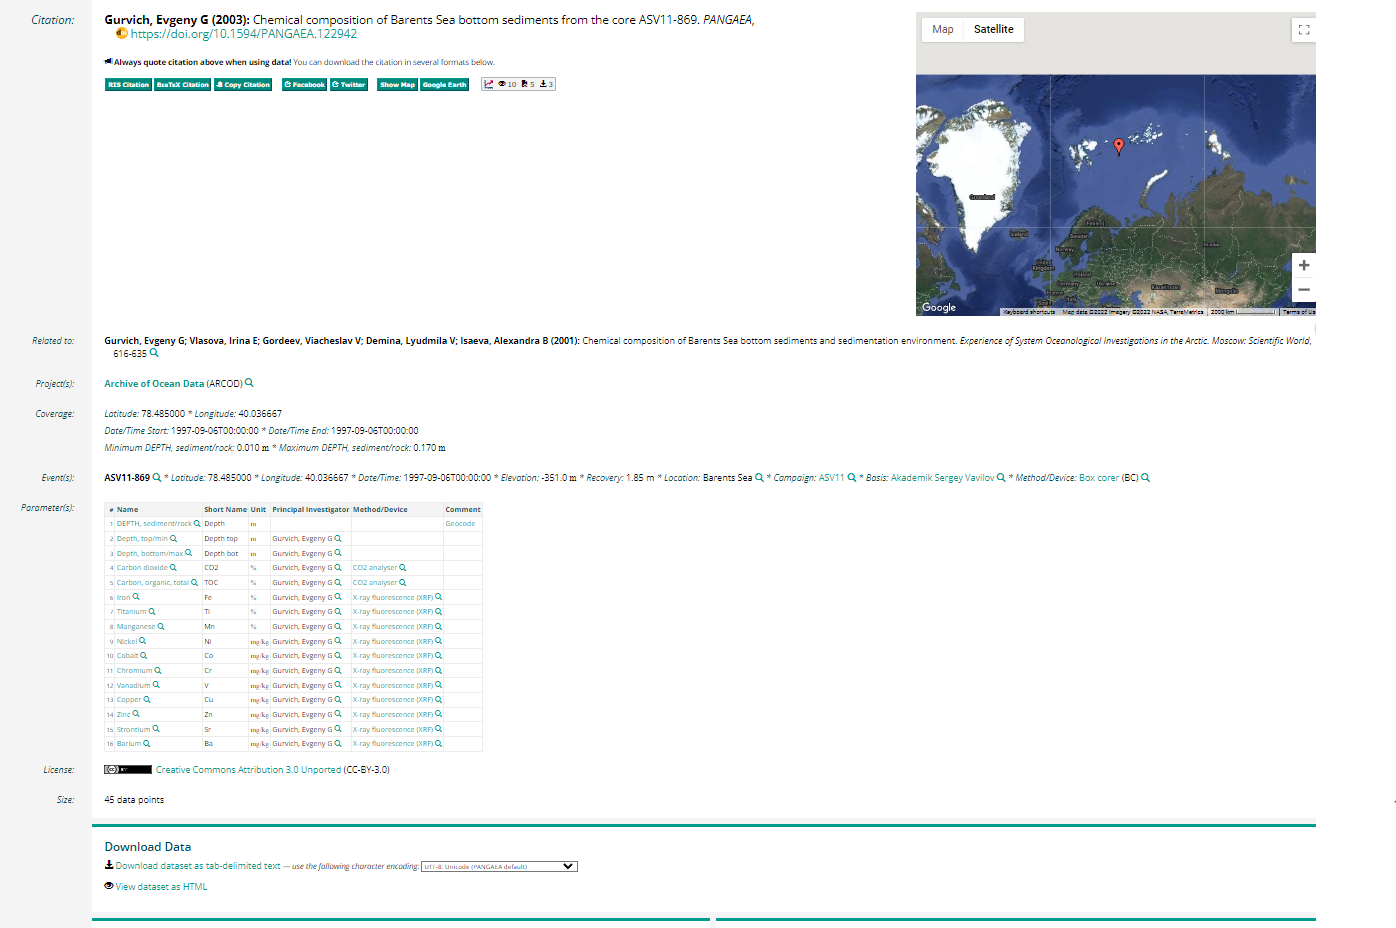
\includegraphics[width=.7\textwidth]{img/abb2_PANGAEA_results.png}
\caption{Abbildung 2: Ergebnispräsentation für den Datensatz
\url{https://doi.org/10.1594/PANGAEA.122942} in PANGAEA}
\end{figure}

\hypertarget{methode}{%
\section{Methode}\label{methode}}

Zwischen den hier vorgestellten Diensten gibt es inhaltliche
Überschneidungen bei den Datenbeständen: Durch das Bereitstellen von
Metadaten über die landing pages sorgt PANGAEA dafür, dass Datensätze
auch in Google Dataset Search indexiert sind. Im Folgenden wird
näherungsweise untersucht, wie erfolgreich Metadaten an Google Dataset
Search übergeben werden. Zu diesem Zweck werden Metadatensätze
verglichen, die in beiden Diensten vorliegen.

\hypertarget{datenerhebung}{%
\subsection{Datenerhebung}\label{datenerhebung}}

Metadaten für Google Dataset Search stammen aus einem Subset der
indexierten Datensätze, das 2020 veröffentlicht wurde (Google Dataset
Search 2020). Das Subset umfasst 17 Metadatenelemente für Datensätze,
für die eine DOI oder ein anderer Identifier vorlag (3.602.027
Datensätze, Stand 16.10.2020). Da PANGAEA DOIs für alle publizierten
Datensätze vergibt, sind diese auch in dem Datensatz enthalten. Zunächst
wurden DOIs identifiziert, die in beiden Datenquellen auftreten (DOIs,
die am 30.10.2022 über die PANGAEA OAI-OMH-Schnittstelle abrufbar waren
sowie DOIs in dem veröffentlichten Subset von Google Dataset Search).
Diese Bedingung trifft auf 364.255 Metadatensätze zu.

Metadaten für 10.000 zufällig ausgewählte PANGAEA-Datensätze wurden am
01.11.2022 über die OAI-PMH-Schnittstelle im Format \emph{PANGAEA
MetaData} abgefragt.\footnote{PANGAEA MetaData:
  \url{http://ws.pangaea.de/schemas/pangaea/MetaData.xsd}}

\hypertarget{analyse}{%
\subsection{Analyse}\label{analyse}}

Zunächst wurde die Nutzung der verfügbaren Metadatenelemente im Subset
von Google Dataset Search analysiert.

Anschließend wurde beispielhaft an zwei Metadatenelementen untersucht,
welche Informationen die beiden vorgestellten Suchdienste für ein
zufällig gewähltes Sample von 10.000 Metadatensätzen vorhalten:

\begin{itemize}
\item
  Informationen über die Methode, die der Datenerhebung zugrunde liegt
  (\emph{method} in PANGAEA und \emph{measurementTechnique} in Google
  Dataset Search)
\item
  Informationen über Fördermittel, die für die Datenerhebung
  bereitgestellt wurden (\emph{funder} in PANGAEA und \emph{funder} in
  Google Dataset Search)
\end{itemize}

Die zwei beschriebenen Metadatenelemente wurden gewählt, da sie für
PANGAEA-Datensätze häufig nicht in der Google Dataset Search vorlagen.
Die Auswahl zielt auf eine Analyse möglicher Probleme beim
Metadatenaustausch ab.

\hypertarget{ergebnisse}{%
\section{Ergebnisse}\label{ergebnisse}}

\hypertarget{metadaten-in-google-dataset-search}{%
\subsection{Metadaten in Google Dataset
Search}\label{metadaten-in-google-dataset-search}}

Abbildung 3 zeigt, wie häufig die verfügbaren Metadatenelemente zur
Beschreibung der PANGAEA-Datensätze in Google Dataset Search genutzt
wurden. Tabelle 1 im Anhang beschreibt die Metadatenelemente und listet
ihre Nutzung im Detail auf.

\begin{figure}[h!]
\centering
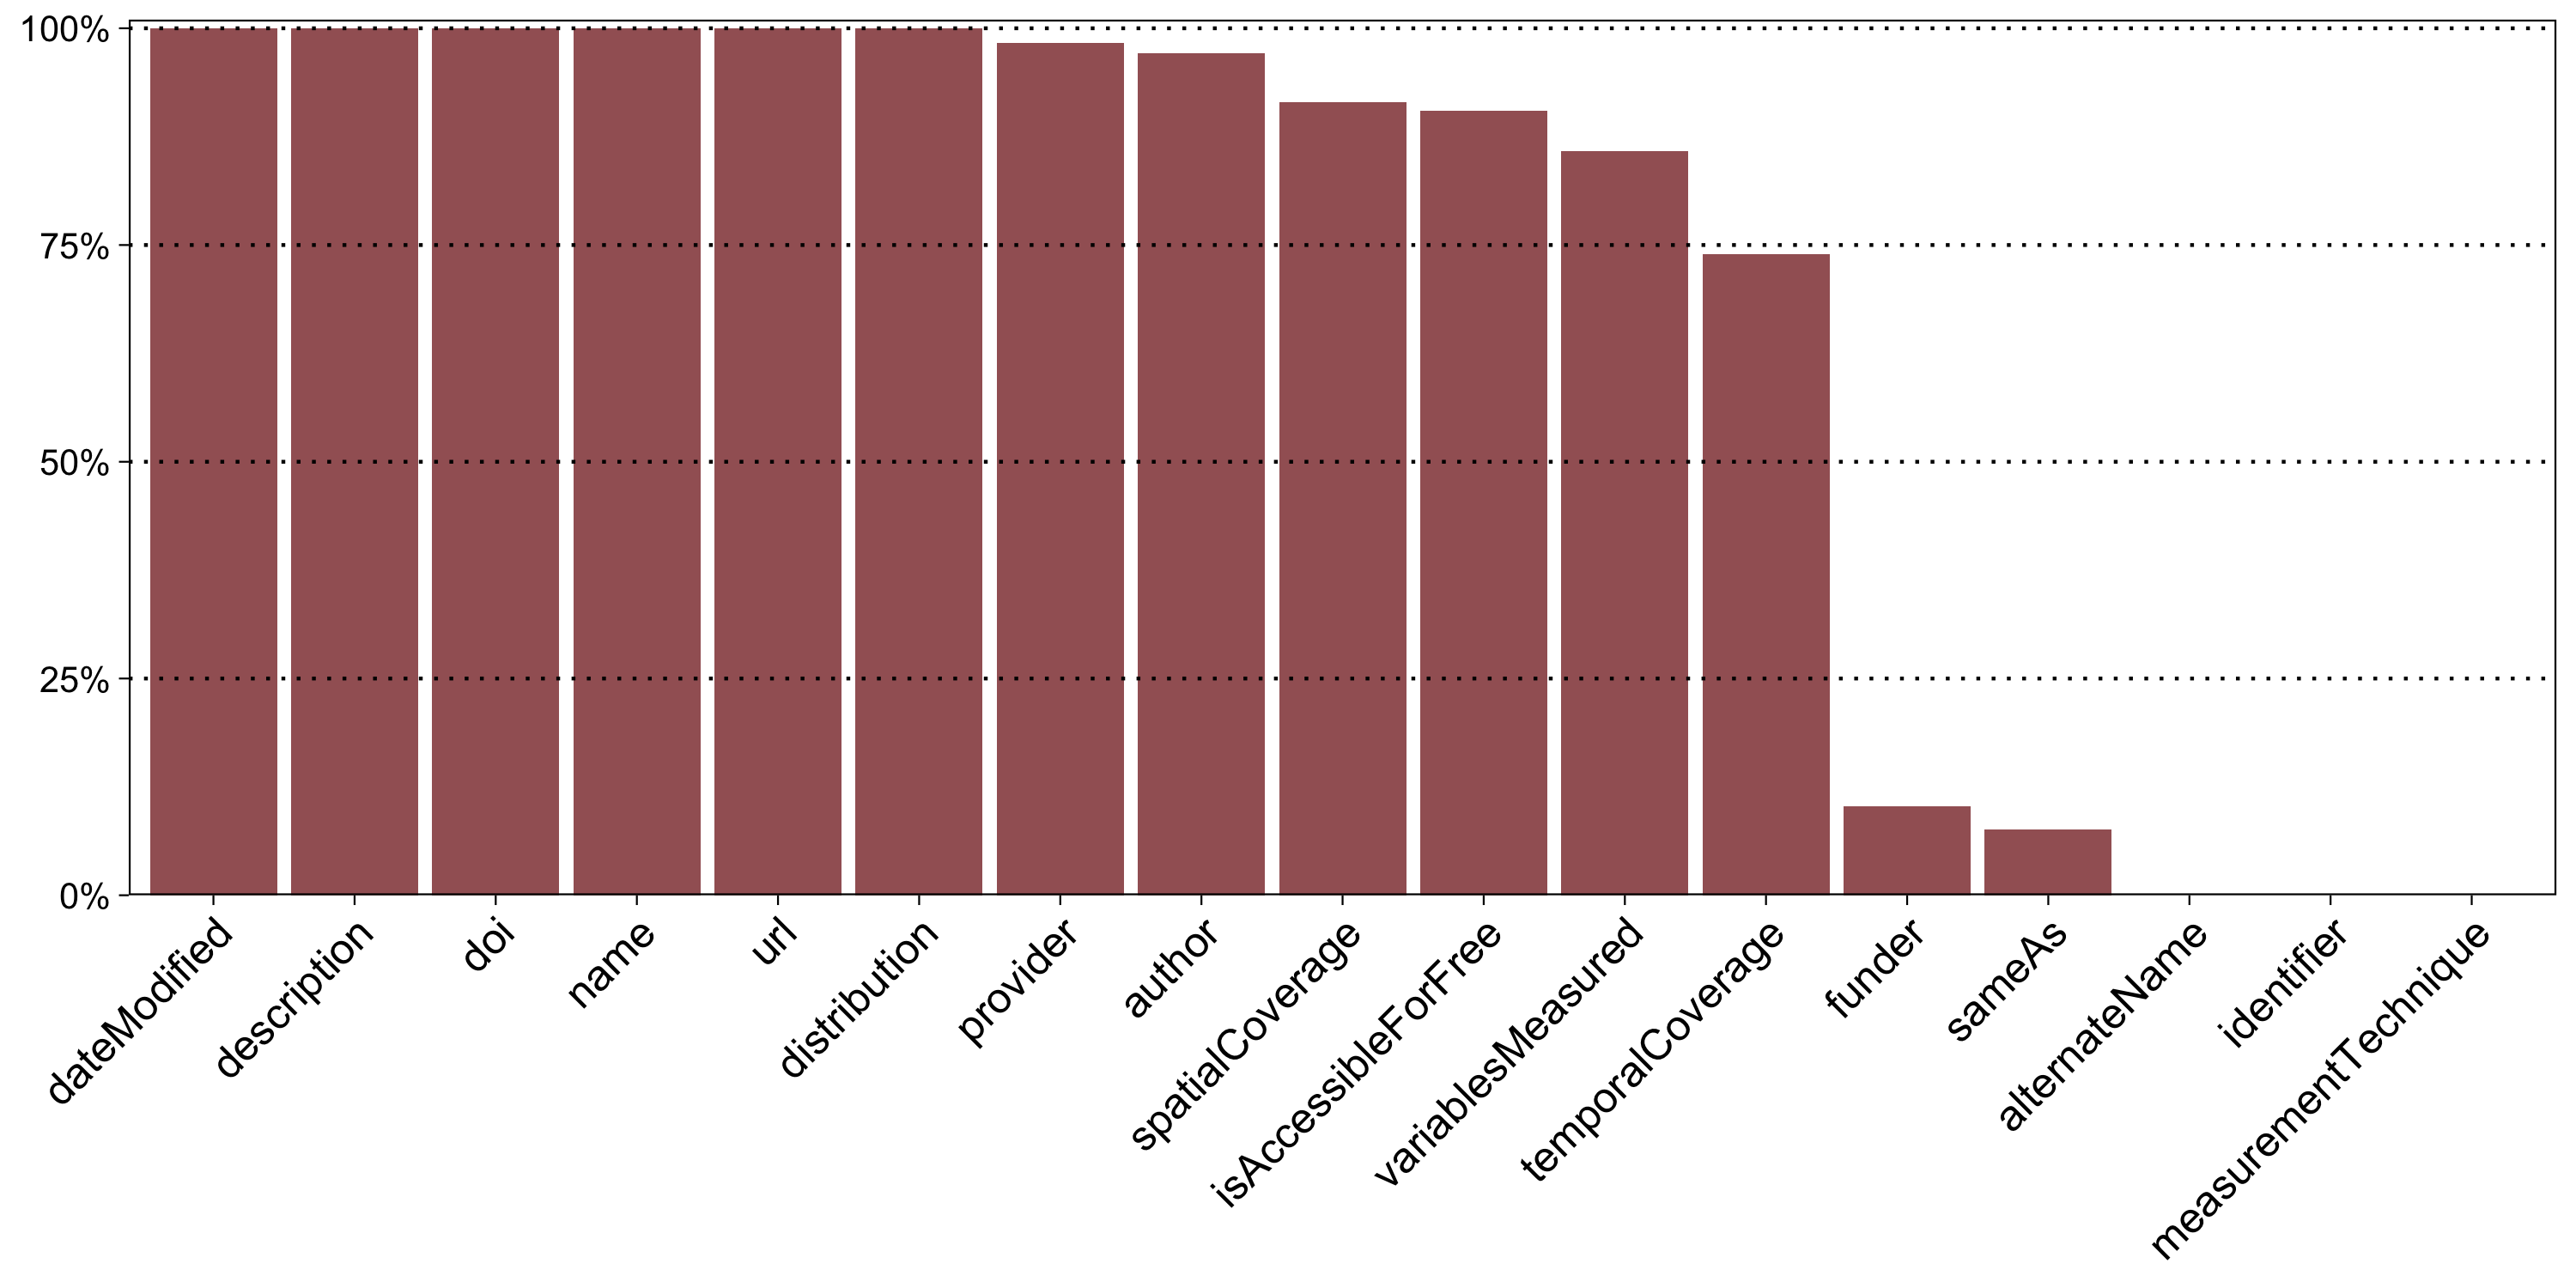
\includegraphics[width=.9\textwidth]{img/abb3_GDS_element_use.png}
\caption{Abbildung 3: Nutzung von Metadatenelementen zur Beschreibung
von PANGAEA-Datensätzen in einem Subset von Google Dataset Search (Stand
16.10.2020)}
\end{figure}

Fünf der in Abbildung 3 dargestellten Metadatenelemente sind in allen
untersuchten Metadatensätzen vorhanden. Dazu zählen neben den zwei
Pflichtelementen \emph{name} und \emph{description} auch
\emph{dateModified}, \emph{doi} und \emph{url}. Fünf weitere Elemente
werden in über 90\,\% der Metadatensätze genutzt: \emph{distribution},
\emph{provider}, \emph{author}, \emph{spatialCoverage} und
\emph{isAccessibleForFree}. Die Elemente \emph{variablesMeasured} und
\emph{temporalCoverage} liegen für die Mehrzahl der Metadatensätze vor.

Im Vergleich deutlich weniger genutzt werden \emph{funder} und
\emph{sameAs}, während drei Metadatenelemente in diesem Bestand nicht
vorkommen (\emph{alternateName}, \emph{identifier},
\emph{measurementTechnique}). Die mangelnde Nutzung einiger dieser
Elemente kann damit erklärt werden, dass sie nicht auf alle Datensätze
zutreffen -- so hat nicht jeder Datensatz alternative Titel, URLs oder
Identifier, die in den Metadaten abgebildet werden können.

\hypertarget{vergleich-zwischen-pangaea-und-google-dataset-search}{%
\subsection{Vergleich zwischen PANGAEA und Google Dataset
Search}\label{vergleich-zwischen-pangaea-und-google-dataset-search}}

Abbildung 4 zeigt anhand eines zufällig gewählten Samples von 10.000
Datensätzen, die in beiden Datenquellen beschrieben sind, Unterschiede
in der Verfügbarkeit von Informationen zu Förderung (\emph{funder}) und
Methoden (\emph{method}).

\begin{figure}[h!]
\centering
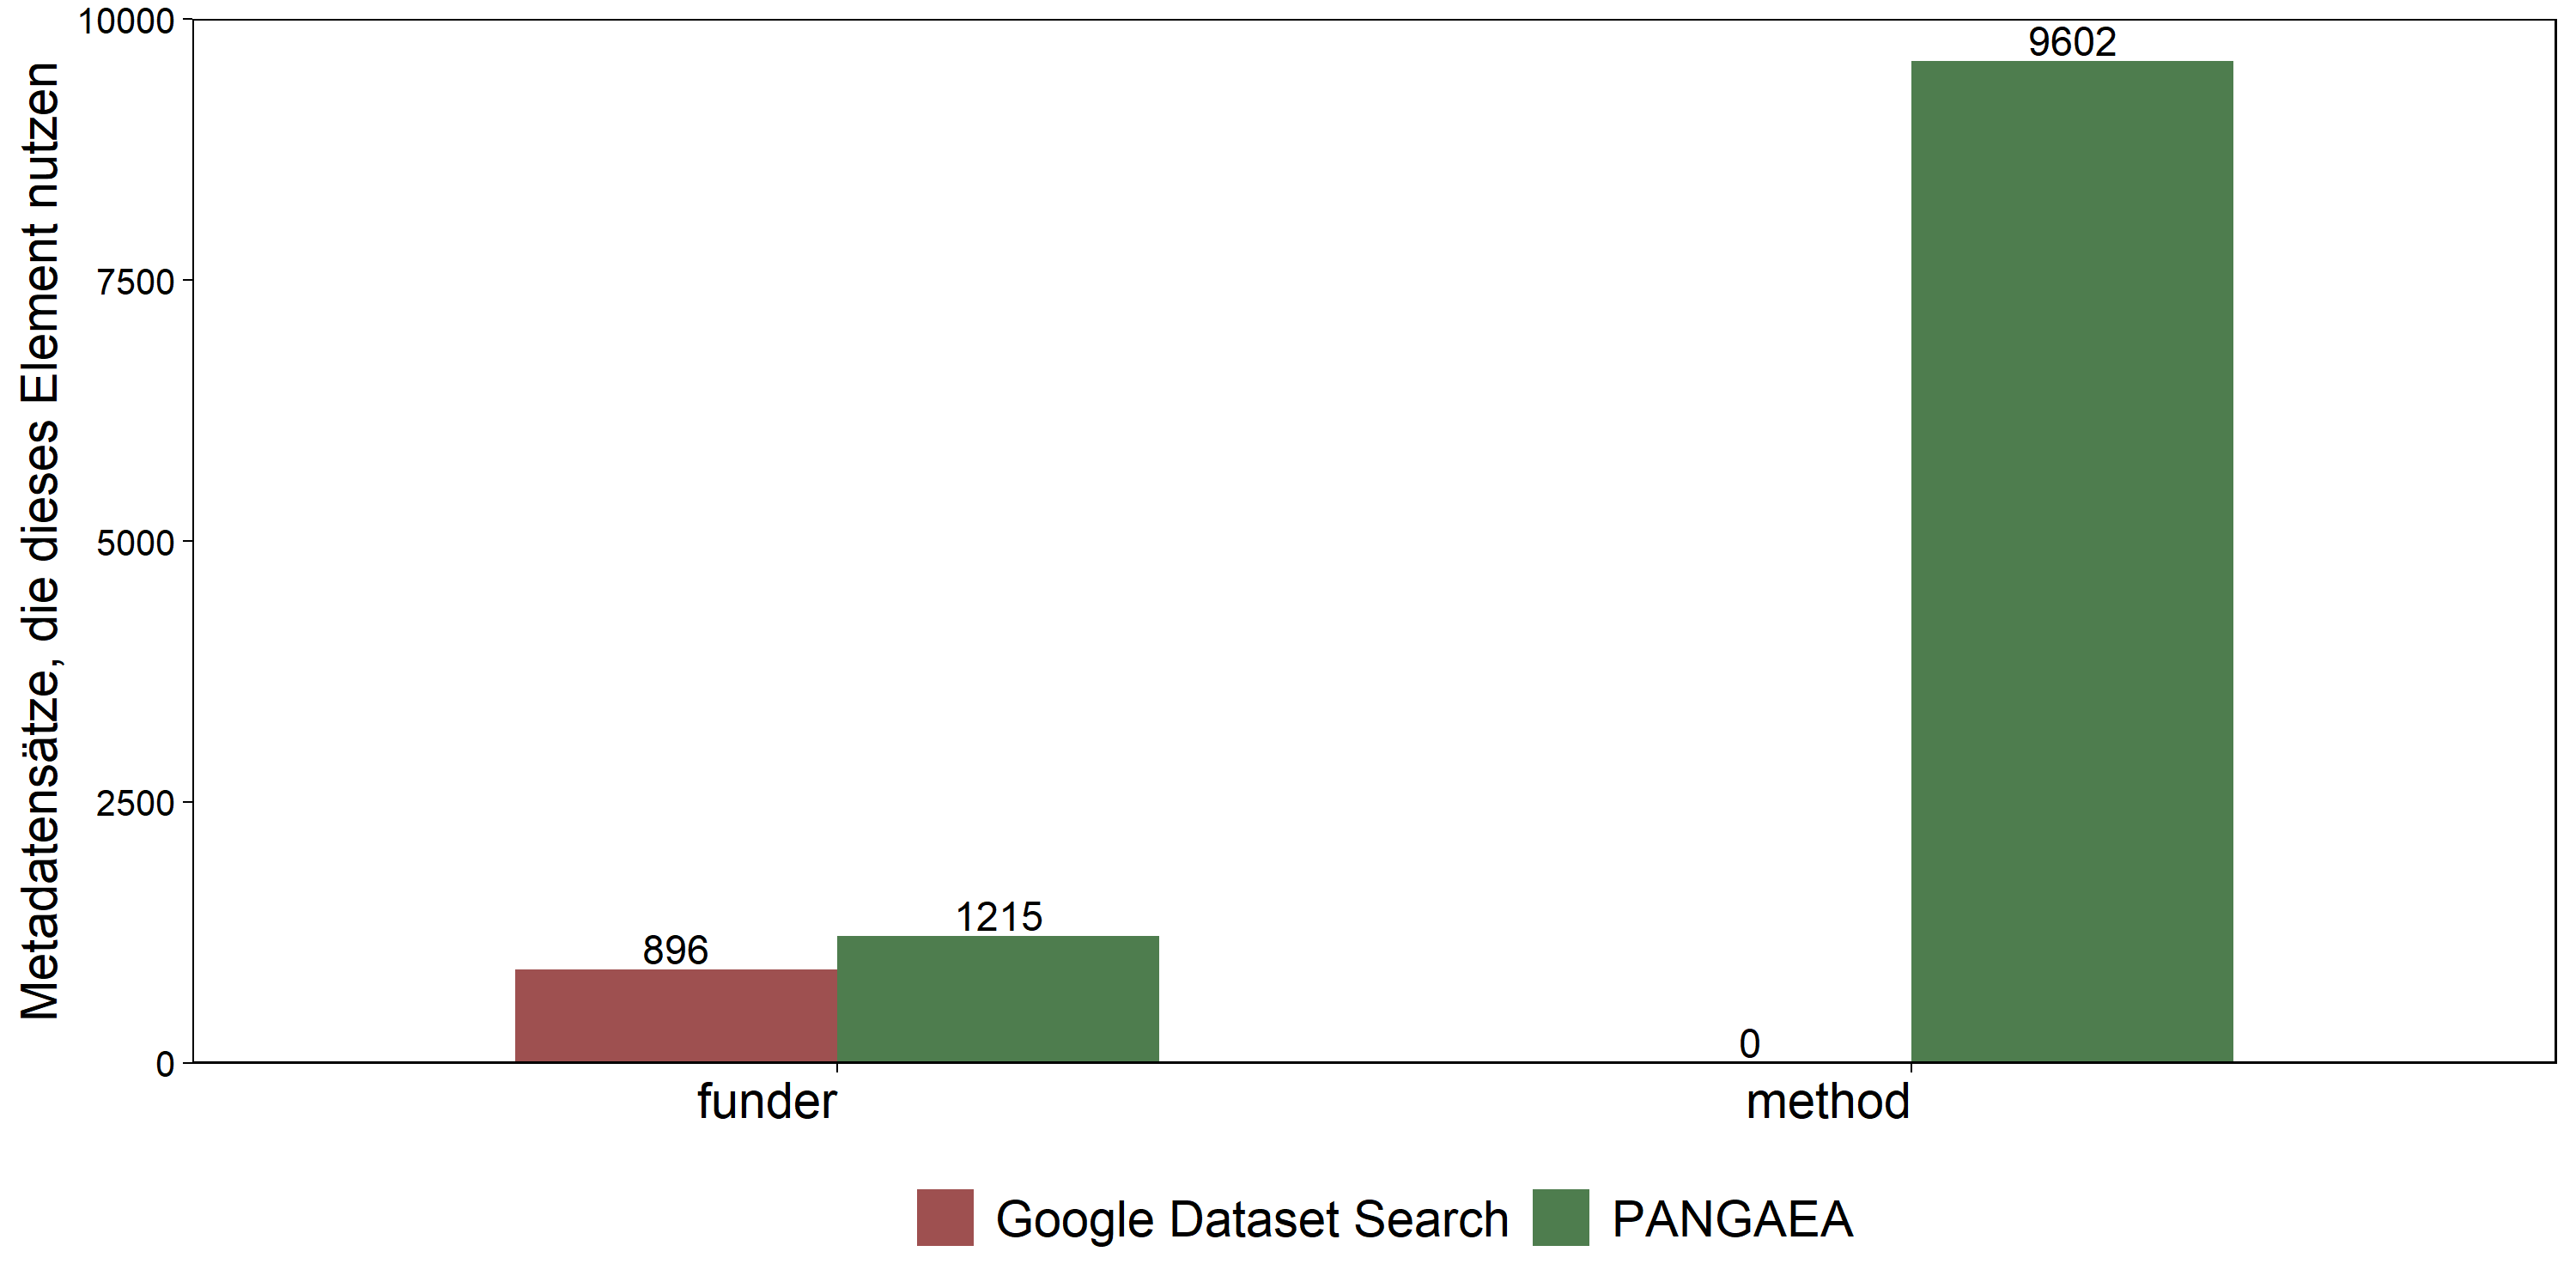
\includegraphics[width=.8\textwidth]{img/abb4_comparative_element_use.png}
\caption{Abbildung 4: Informationen zu Förderern und Methoden in Google
Dataset Search und PANGAEA (Sample von 10.000 Metadatensätzen)}
\end{figure}

Informationen zu Fördermitteln sind in PANGAEA etwas häufiger vorhanden
als in Google Dateset Search; aber auch in PANGAEA sind diese Angaben
nicht weit verbreitet. Unterschiede zwischen den beiden DR-Systemen
zeigen sich besonders deutlich in der Verfügbarkeit von Informationen zu
Methoden, die der Datenerhebung zugrunde liegen. Während diese Angaben
in PANGAEA für fast alle Datensätze vorliegen (96,02\,\% ; n = 9.602),
fehlen sie in Google Dataset Search komplett.

\hypertarget{diskussion}{%
\section{Diskussion}\label{diskussion}}

DR ist ein schnell wachsendes Forschungsfeld innerhalb von IR, was
sicher von der steigenden Anzahl verfügbarer Datensätze durch
Open-Science-Initiativen beeinflusst wird.\\
DR-Systeme orientieren sich bisher stark an IR-Systemen, werden jedoch
nicht immer den objekttypspezifischen Anforderungen gerecht, die
Datensätze mit sich bringen können. Zu den aktuellen Herausforderungen
im Bereich DR zählt das Fehlen von Suchansätzen, die über Keywordsuche
und Filteroptionen hinausgehen, sowie der Fokus auf strukturierte
Metadaten, da Metadaten für Forschungsdaten nicht immer in ausreichendem
Umfang vorliegen oder Qualitätsanforderungen beziehungsweise
Informationsbedürfnissen entsprechen. Auch stellt der Mangel an
spezialisierten Evaluationskonzepten für DR-Systeme ein Problem dar. Nur
wenige Repositorienbetreiber*innen haben ihr DR-System in der
Vergangenheit evaluiert. Dadurch fehlen beispielsweise gesicherte
Erkenntnisse über die Eignung des DR-Systems für das erfolgreiche
Auffinden geeigneter Datensätze, und damit auch Ansätze für die
Verbesserung des Dienstes.

Die Suche nach Daten unterscheidet sich in einigen Aspekten von der
Suche nach Textpublikationen. Darum ist es wichtig, das
Informationsverhalten von Datensuchenden gezielt zu betrachten. In den
vergangenen Jahren gab es eine Reihe von Vorhaben mit dieser
Zielsetzung, vor allem in den Sozialwissenschaften. Die Ergebnisse
zeigen, dass Datensuchende auf verschiedene Quellen zurückgreifen, auch
in Kombination. Dabei nutzen sie nicht nur spezialisierte
Datensuchdienste, sondern auch persönliche Kontakte oder Verweise in
Textpublikationen. Auch Websuchmaschinen werden bei der Datensuche
häufig genutzt. Bei der Nutzung von Websuchmaschinen fallen Muster wie
das Ergänzen der Suchanfrage um Begriffe wie \enquote*{data} oder die
Namen bekannter Datenrepositorien auf. Suchanfragen in spezialisierten
Datensuchdiensten beinhalten häufig Einschränkungen, die sich auf
bestimmte Eigenschaften von Datensätzen beziehen, beispielsweise die
räumliche oder zeitliche Abdeckung. Eine verbreitete Strategie scheint
das bewusste Formulieren kurzer Anfragen zu sein, um lange Trefferlisten
zu erzeugen, die dann manuell geprüft werden. Insgesamt sollten
spezialisierte Datensuchdienste stärker beworben werden, damit
Forschende wissen, wo sie geeignete Daten finden können.

Wie für die Suche nach Textpublikationen haben sich verschiedene Arten
von Suchdiensten herausgebildet, die sich beispielsweise im Umfang der
indexierten Datenquellen (zentral -- dezentral) und dem disziplinären
Fokus (disziplinspezifisch -- disziplinübergreifend) unterscheiden.
Disziplinspezifische und zentrale DR-Systeme wie PANGAEA können stärker
als disziplinübergreifende oder dezentrale Dienste (zum Beispiel Google
Dataset Search) auf spezielle Informationsbedürfnisse ihrer Nutzenden
eingehen, was sich beispielsweise an den durchsuchbaren Metadaten, den
zur Verfügung gestellten Sucheinstiegen und der Präsentation der
Ergebnisse zeigt. Der Vorteil von dezentralen Diensten ist, dass sie
mehrere Datenbestände aggregieren und durchsuchbar machen. Sie können
zwar nicht auf spezielle Informationsbedürfnisse eingehen, schaffen aber
schwellenarme und bestandsübergreifende Angebote für DR. Dadurch tragen
sie zu einer besseren Sichtbarkeit von Datensätzen bei, was auch im
Interesse von Repositorien wie PANGAEA ist.

Metadaten der Datensätze, die in PANGAEA publiziert wurden, werden auch
von Google Dataset Search indexiert. Der Metadatenaustausch zwischen den
Diensten ist sehr effektiv, denn der Beschreibungsgrad von
PANGAEA-Datensätzen in Google Datasest Search ist verglichen mit anderen
Datenquellen überdurchschnittlich gut. So sind Informationen über
Autor*innen nur für 14,2\,\% aller Datensätze im untersuchten Subset von
Google Dataset Search vorhanden (Benjelloun, Chen und Noy 2020), während
die Angabe für mehr als 90\,\% der PANGAEA-Datensätze vorliegen. Die
Analyse zeigte jedoch, dass Informationen zu Erhebungsmethoden nicht in
vollständigem Umfang weitergegeben werden. Eine mögliche Erklärung dafür
könnte sein, dass PANGAEA zu dem Zeitpunkt, an dem das Subset erstellt
wurde (2020), das Mapping zwischen dem Metadatenschemata PANGAEA
MetaData und schema.org noch nicht optimiert hatte. Dadurch könnten
Informationen zur angewendeten Methode, die intern vorhanden sind, nicht
in die landing pages eingebettet und darum nicht von Crawls erfasst
werden.

Metadatenelemente, die in Google Dataset Search genutzt werden, sind
überwiegend beschreibend und nicht sehr umfangreich. Sie dienen der
Auffindbarkeit, indem identifizierende Eigenschaften (zum Beispiel
Titel, Autor*in) sowie der Kontext (zum Beispiel räumliche und zeitliche
Abdeckung) abgebildet werden. Demgegenüber können Forschungsdaten in
PANGAEA durch ein detailliertes Metadatenschema deutlich präziser
beschrieben werden. Darüber hinaus werden bei PANGAEA kontrollierte
Vokabulare eingesetzt, die semantische Bezüge zwischen Datensätzen
herstellen und die Interoperabilität verbessern.

\hypertarget{fazit}{%
\section{Fazit}\label{fazit}}

Durch die zunehmende Verfügbarkeit von publizierten Forschungsdaten
gewinnt Dataset Retrieval an Bedeutung. Aktuell findet das Thema viel
Aufmerksamkeit in der Forschung, zum Beispiel mit Blick auf die
Anpassung von Suchdiensten an objekttypspezifische Besonderheiten von
Forschungsdaten oder das Informationsverhalten von Datensuchenden. Auch
wenn der Metadatenaustausch nicht immer reibungslos abläuft, entwickelt
sich nach und nach ein Ökosystem ineinandergreifender DR-Systeme. Einige
sind stark an die Bedürfnisse von Datensuchenden angepasst, während
andere mehrere Datenbestände aggregieren und schwellenarme Sucheinstiege
anbieten. DR-Systeme vereinfachen das Auffinden von Forschungsdaten für
die Nachnutzung und tragen so zum Erfolg von Open-Science-Initiativen
bei.

\hypertarget{limitationen}{%
\subsection{Limitationen}\label{limitationen}}

Der Vergleich der hier vorgestellten Dienste basiert unter anderem auf
einem Subset, das Google Dataset Search 2020 veröffentlicht und seither
nicht aktualisiert hat. Metadaten von PANGAEA wurden demgegenüber 2022
gesammelt. Aufgrund dieser zeitlichen Differenz muss der Vergleich als
ungefähre Annäherung gelten, die verdeutlichen soll, dass der
Metadatenaustausch zwischen Diensten nicht immer reibungslos abläuft.

\pagebreak

\hypertarget{anhang-a}{%
\section{Anhang A}\label{anhang-a}}

\begin{table}[h!]
    \caption{Tabelle 1: Beschreibung der Metadatenelemente in Google Dataset Search und deren Vorkommen für PANGAEA-Datensätze}
    \begin{tabular}{lp{6cm}>{\raggedleft\arraybackslash}p{2cm}>{\raggedleft\arraybackslash}p{2cm}}
    \toprule
    \textbf{Element}             & \textbf{Beschreibung}                                                                 & \textbf{Verwendung \newline (total)} & \textbf{Verwendung \newline (anteilig)} \\ \midrule
    dateModified         & Zeitpunkt, zu dem der Datensatz zuletzt bearbeitet wurde                     & 36.4255            & 100\,\%                \\ \midrule
    description          & Beschreibung des Datensatzes                                                 & 36.4255            & 100\,\%                \\ \midrule
    doi                  & DOI des Datensatzes                                                          & 36.4255            & 100\,\%                \\ \midrule
    name                 & Titel des Datensatzes                                                        & 36.4255            & 100\,\%                \\ \midrule
    url                  & URL des Datensatzes                                                          & 36.4255            & 100\,\%                \\ \midrule
    distribution         & Angaben zum Download des Datensatzes                                         & 36.4221            & 99,99\,\%              \\ \midrule
    provider             & Organisation, die den Datensatz zur Verfügung stellt                         & 358.051            & 98,3\,\%               \\ \midrule
    author               & Autor*innen des Datensatzes                                                  & 353.825            & 97,14\,\%              \\ \midrule
    spatialCoverage      & Räumliche Abdeckung des Datensatzes                                          & 333.179            & 91,47\,\%              \\ \midrule
    isAccessibleForFree  & Indikator, der angibt, ob der Datensatz frei verfügbar ist                   & 329.631            & 90,49\,\%              \\ \midrule
    variablesMeasured    & Gemessene Variablen, die im Datensatz repräsentiert werden                   & 312.664            & 85,84\,\%              \\ \midrule
    temporalCoverage     & Zeitliche Abdeckung des Datensatzes                                          & 269.335            & 73,49\,\%              \\ \midrule
    funder               & Fördermittel, die zur Erhebung des Datensatzes zur Verfügung gestellt wurden & 37.269             & 10,23\,\%              \\ \midrule
    sameAs               & Alternative URL des Datensatzes                                              & 27.666             & 7,6\,\%                \\ \midrule
    alternateName        & Alternativer Titel des Datensatzes                                           & 0                  & 0\,\%                  \\ \midrule
    identifier           & Identifier (außer DOI) des Datensatzes                                       & 0                  & 0\,\%                  \\ \midrule
    measurementTechnique & Methode, die zur Messung der repräsentierten Variablen angewendet wurde      & 0                  & 0\,\%                  \\ 
    \bottomrule
    \end{tabular}
\end{table}

\pagebreak

\section{Literaturverzeichnis}\label{literaturverzeichnis}

Benjelloun, Omar, Shiyu Chen, und Natasha Noy. 2020. \enquote{Google
Dataset Search by the Numbers.} In \emph{The Semantic Web -- ISWC 2020},
edited by Jeff Pan, Valentina Tamma, Claudia d'Amato, Krzysztof
Janowicz, Bo Fu, Axel Polleres, Oshani Seneviratne, und Lalana Kagal,
667--82. Lecture Notes in Computer Science. Springer International
Publishing. \url{https://doi.org/10.1007/978-3-030-62466-8_41}.

Borst, Timo, und Fidan Limani. 2020. \enquote{Patterns for Searching
Data on the Web Across Different Research Communities.} \emph{LIBER
Quarterly} 30 (1): 1--21. \url{https://doi.org/10.18352/lq.10317}.

Brickley, Dan, Matthew Burgess, und Natasha Noy. 2019. \enquote{Google
Dataset Search: Building a Search Engine for Datasets in an Open Web
Ecosystem.} In \emph{The World Wide Web Conference}, 1365--75. New York:
Association for Computing Machinery.
\url{https://doi.org/10.1145/3308558.3313685}.

Canino, Adrienne. 2019. \enquote{Deconstructing Google Dataset Search.}
\emph{Public Services Quarterly} 15 (3): 248--55.
\url{https://doi.org/10.1080/15228959.2019.1621793}.

Carevic, Zeljko, Dwaipayan Roy, und Philipp Mayr. 2020.
\enquote{Characteristics of Dataset Retrieval Sessions: Experiences from
a Real-Life Digital Library.} In \emph{Digital Libraries for Open
Knowledge}, edited by Mark Hall, Tanja Merčun, Thomas Risse, und Fabien
Duchateau, 185--93. Lecture Notes in Computer Science. Springer.
\url{https://doi.org/10.1007/978-3-030-54956-5_14}.

Chapman, Adriane, Elena Simperl, Laura Koesten, George Konstantinidis,
Luis-Daniel Ibáñez, Emilia Kacprzak, und Paul Groth. 2020.
\enquote{Dataset Search: A Survey.} \emph{The VLDB Journal} 29 (1):
251--72. \url{https://doi.org/10.1007/s00778-019-00564-x}.

Chen, Jinchi, Xiaxia Wang, Gong Cheng, Evgeny Kharlamov, und Yuzhong Qu.
2019. \enquote{Towards More Usable Dataset Search: From Query
Characterization to Snippet Generation.} In \emph{Proceedings of the
28th ACM International Conference on Information and Knowledge
Management}, 2445--48. New York: Association for Computing Machinery.
\url{https://doi.org/10.1145/3357384.3358096}.

Dede Şener, Duygu, Hasan Ogul, und Selen Basak. 2022.
\enquote{Text-Based Experiment Retrieval in Genomic Databases.}
\emph{Journal of Information Science}, 01655515221118670.
\url{https://doi.org/10.1177/01655515221118670}.

Devaraju, Anusuriya, und Shlomo Berkovsky. 2018. \enquote{A Hybrid
Recommendation Approach for Open Research Datasets.} In
\emph{Proceedings of the 26th Conference on User Modeling, Adaptation
and Personalization}, 207--11. New York, NY: Association for Computing
Machinery. \url{https://doi.org/10.1145/3209219.3209250}.

Diepenbroek, Michael, Hannes Grobe, Manfred Reinke, Uwe Schindler,
Reiner Schlitzer, Rainer Sieger, und Gerold Wefer. 2002.
\enquote{PANGAEA---an Information System for Environmental Sciences.}
\emph{Computers \& Geosciences} 28 (10): 1201--10.
\url{https://doi.org/10.1016/S0098-3004(02)00039-0}.

Diepenbroek, Michael, Uwe Schindler, Robert Huber, Stéphane Pesant,
Markus Stocker, Janine Felden, Melanie Buss, und Matthias Weinrebe.
2017. \enquote{Terminology Supported Archiving and Publication of
Environmental Science Data in PANGAEA.} \emph{Journal of Biotechnology}
261: 177--86. \url{https://doi.org/10.1016/j.jbiotec.2017.07.016}.

Friedrich, Tanja. 2020. \enquote{Looking for Data.} Dissertation,
Berlin: Humboldt Universität zu Berlin.
\url{https://doi.org/10.18452/22173}.

Google Dataset Search. 2020. \enquote{Dataset Search: Metadata for
Datasets.}
\url{https://www.kaggle.com/datasets/1d97de37cb96c2c62182d22bf5924e0371933002bb7e5c46ba205b8a88de2e21}.

Gregory, Kathleen, Helena Cousijn, Paul Groth, Andrea Scharnhorst, und
Sally Wyatt. 2020. \enquote{Understanding Data Search as a
Socio-Technical Practice.} \emph{Journal of Information Science} 46 (4):
459--75. \url{https://doi.org/10.1177/0165551519837182}.

Gregory, Kathleen, Paul Groth, Helena Cousijn, Andrea Scharnhorst, und
Sally Wyatt. 2019. \enquote{Searching Data: A Review of Observational
Data Retrieval Practices in Selected Disciplines.} \emph{Journal of the
Association for Information Science and Technology} 70 (5): 419--32.
\url{https://doi.org/10.1002/asi.24165}.

Gregory, Kathleen, Paul Groth, Andrea Scharnhorst, und Sally Wyatt.
2020. \enquote{Lost or Found? Discovering Data Needed for Research.}
\emph{Harvard Data Science Review} 2 (2).
\url{https://doi.org/10.1162/99608f92.e38165eb}.

Ibáñez, Luis-Daniel, und Elena Simperl. 2022. \enquote{A Comparison of
Dataset Search Behaviour of Internal Versus Search Engine Referred
Sessions.} In \emph{ACM SIGIR Conference on Human Information
Interaction and Retrieval}, 158--68. New York: Association for Computing
Machinery. \url{https://doi.org/10.1145/3498366.3505821}.

Kacprzak, Emilia, Laura Koesten, Luis-Daniel Ibáñez, Tom Blount, Jeni
Tennison, und Elena Simperl. 2019. \enquote{Characterising Dataset
Search---An Analysis of Search Logs and Data Requests.} \emph{Journal of
Web Semantics} 55: 37--55.
\url{https://doi.org/10.1016/j.websem.2018.11.003}.

Kacprzak, Emilia, Laura Koesten, Luis-Daniel Ibáñez, Elena Simperl, und
Jeni Tennison. 2017. \enquote{A Query Log Analysis of Dataset Search.}
In \emph{Web Engineering}, edited by Jordi Cabot, Roberto De Virgilio,
und Riccardo Torlone, 429--36. Lecture Notes in Computer Science.
Springer. \url{https://doi.org/10.1007/978-3-319-60131-1_29}.

Kern, Dagmar, und Brigitte Mathiak. 2015. \enquote{Are There Any
Differences in Data Set Retrieval Compared to Well-Known Literature
Retrieval?} In \emph{Research and Advanced Technology for Digital
Libraries}, edited by Sarantos Kapidakis, Cezary Mazurek, und Marcin
Werla, 197--208. Lecture Notes in Computer Science. Springer.
\url{https://doi.org/10.1007/978-3-319-24592-8_15}.

Khalsa, SiriJodha, Peter Cotroneo, und Mingfang Wu. 2018. \enquote{A
Survey of Current Practices in Data Search Services.}
\url{https://doi.org/10.17632/7j43z6n22z.1}.

Koesten, Laura M., Emilia Kacprzak, Jenifer F. A. Tennison, und Elena
Simperl. 2017. \enquote{The Trials and Tribulations of Working with
Structured Data: -a Study on Information Seeking Behaviour.} In
\emph{Proceedings of the 2017 CHI Conference on Human Factors in
Computing Systems}, 1277--89. New York: Association for Computing
Machinery. \url{https://doi.org/10.1145/3025453.3025838}.

Krämer, Thomas, Andrea Papenmeier, Zeljko Carevic, Dagmar Kern, und
Brigitte Mathiak. 2021. \enquote{Data-Seeking Behaviour in the Social
Sciences.} \emph{International Journal on Digital Libraries} 22 (2):
175--95. \url{https://doi.org/10.1007/s00799-021-00303-0}.

Kunze, Sven, und Sören Auer. 2013. \enquote{Dataset Retrieval.} In,
1--8. \url{https://doi.org/10.1109/ICSC.2013.12}.

Luk, Robert. 2022. \enquote{Why Is Information Retrieval a Scientific
Discipline?} \emph{Foundations of Science} 27 (2): 427--53.
\url{https://doi.org/10.1007/s10699-020-09685-x}.

Masson, Arnaud, Guido De Marchi, Bruno Merin, Maria Sarmiento, David
Wenzel, und Beatriz Martinez. 2021. \enquote{Google Dataset Search and
DOI for Data in the ESA Space Science Archives.} \emph{Advances in Space
Research} 67 (8): 2504--16.
\url{https://doi.org/10.1016/j.asr.2021.01.035}.

Meadow, Charles, Bert Boyce, Donald Kraft, und Carol Barry. 2007.
\emph{Text Information Retrieval Systems}. Cambridge, MA: Academic
Press.

Noy, Natasha, und Omar Benjelloun. 2020. \enquote{An Analysis of Online
Datasets Using Dataset Search.} \emph{Google AI Blog}.
\url{http://ai.googleblog.com/2020/08/an-analysis-of-online-datasets-using.html}.

Roy, Dwaipayan, Zeljko Carevic, und Philipp Mayr. 2022.
\enquote{Studying Retrievability of Publications und Datasets in an
Integrated Retrieval System.} In \emph{Proceedings of the 22nd ACM/IEEE
Joint Conference on Digital Libraries}, 1--9. New York, NY: Association
for Computing Machinery. \url{https://doi.org/10.1145/3529372.3530931}.

Sanderson, Mark, und Bruce Croft. 2012. \enquote{The History of
Information Retrieval Research.} \emph{Proceedings of the IEEE} 100
(Special Centennial Issue): 1444--51.
\url{https://doi.org/10.1109/JPROC.2012.2189916}.

Sun, Guangyuan, Tanja Friedrich, Kathleen Gregory, und Brigitte Mathiak.
2022. \enquote{Are We Building the Data Discovery Infrastructure
Researchers Want? Comparing Perspectives of Support Specialists und
Researchers.} arXiv. \url{https://doi.org/10.48550/arXiv.2209.14655}.

Wang, Xu, Zhisheng Huang, und Frank van Harmelen. 2020.
\enquote{Evaluating Similarity Measures for Dataset Search.} In
\emph{Web Information Systems Engineering -- WISE 2020}, edited by
Zhisheng Huang, Wouter Beek, Hua Wang, Rui Zhou, und Yanchun Zhang,
38--51. Springer. \url{https://doi.org/10.1007/978-3-030-62008-0_3}.

Wu, Mingfang, Fotis Psomopoulos, Siri Jodha Khalsa, und Anita de Waard.
2019. \enquote{Data Discovery Paradigms: User Requirements and
Recommendations for Data Repositories.} \emph{Data Science Journal} 18
(1): 3. \url{https://doi.org/10.5334/dsj-2019-003}.

%autor
\begin{center}\rule{0.5\linewidth}{0.5pt}\end{center}

\textbf{Dorothea Strecker} ist Wissenschaftliche Mitarbeiterin im
Projekt re3data COREF am Institut für Bibliotheks- und
Informationswissenschaft der Humboldt-Universität zu Berlin.

\end{document}